\chapter{Security of Connect IQ store}
\section{Preliminary analysis}
\begin{figure}[h]
    \centering
    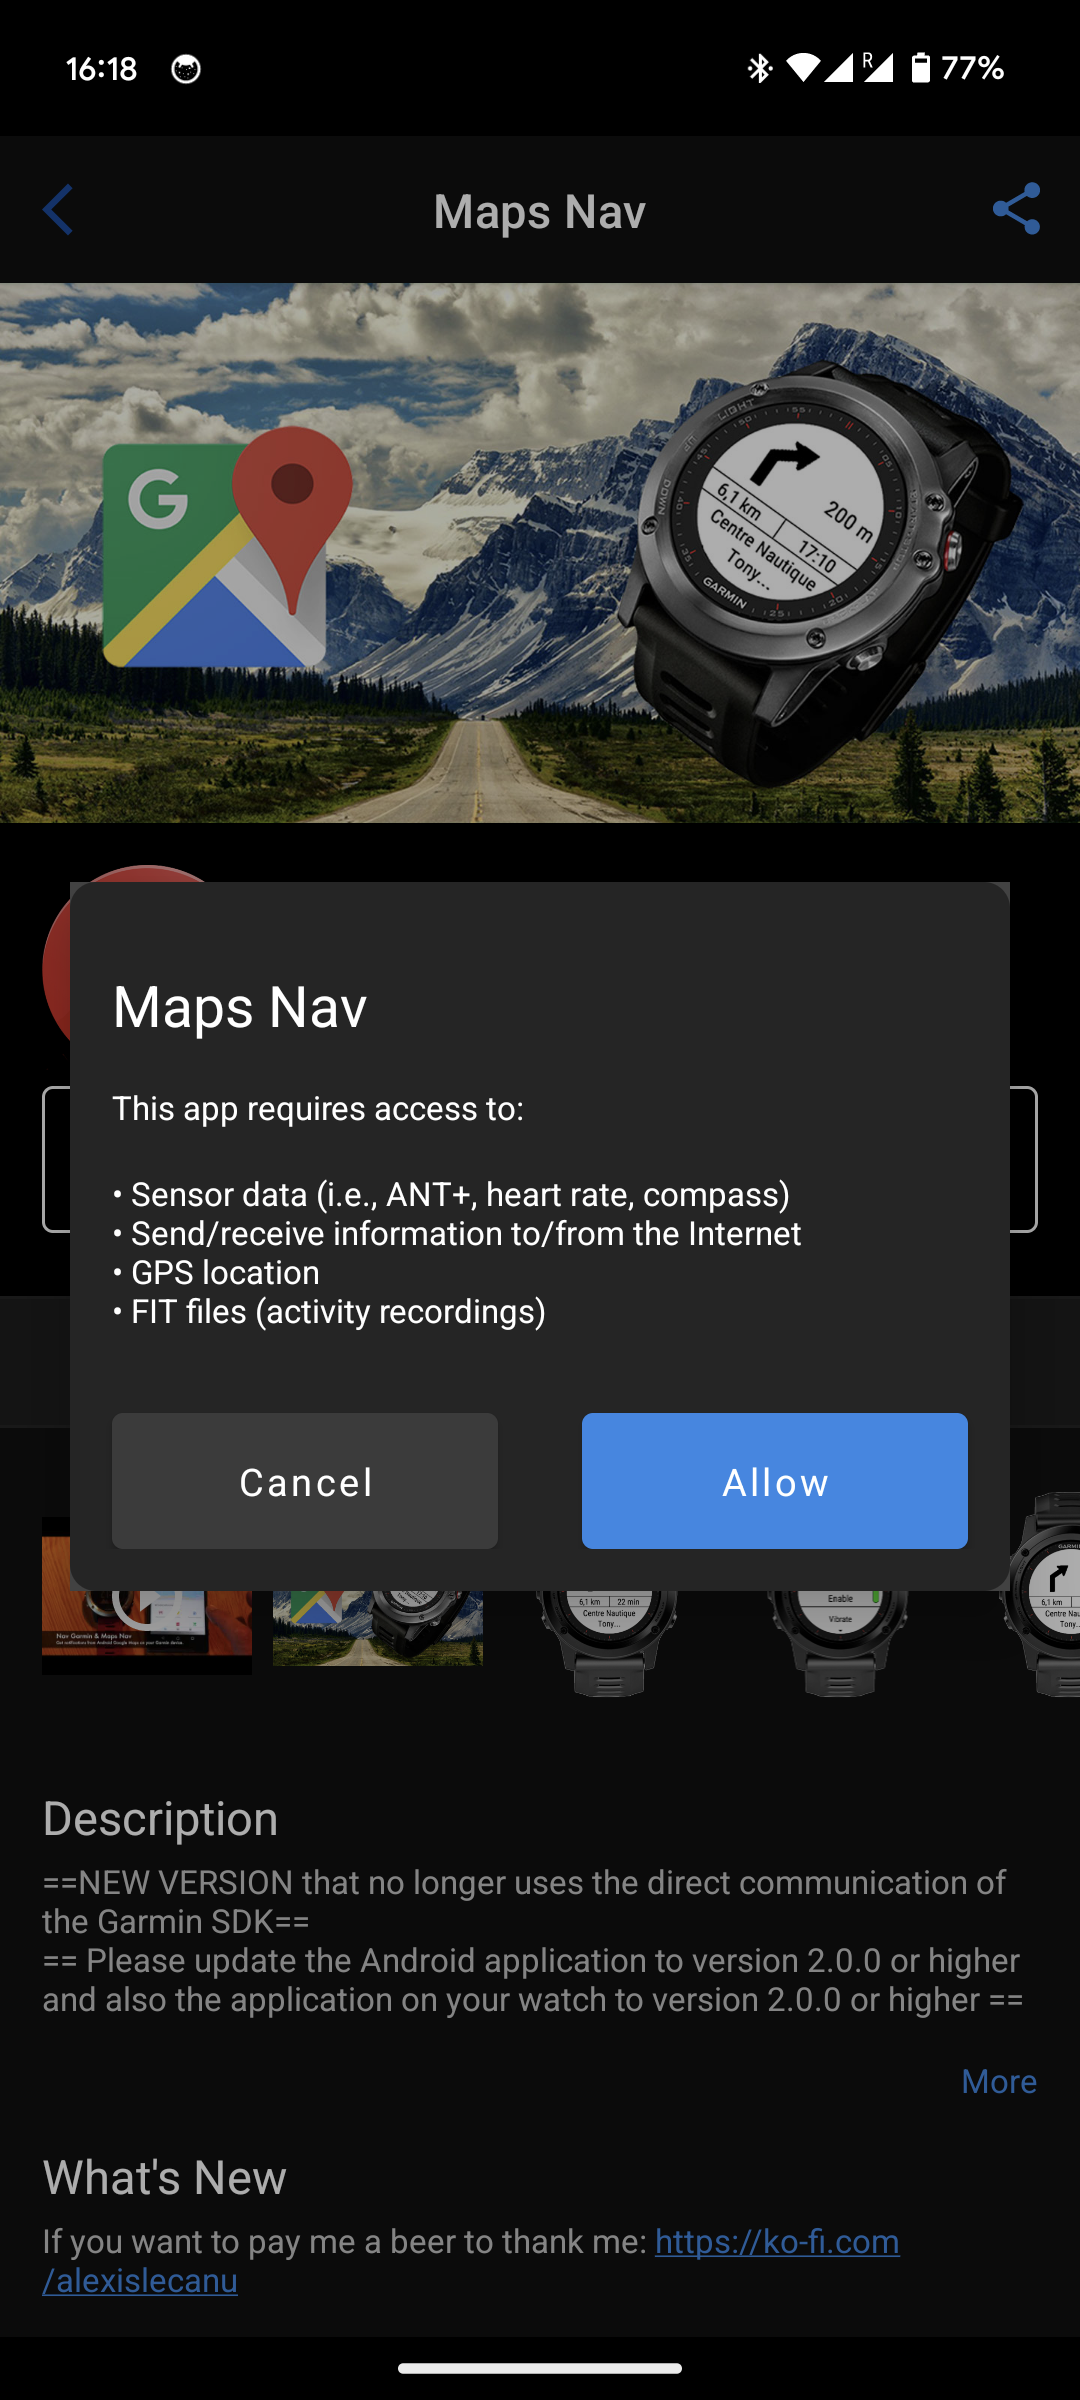
\includegraphics[width=0.3\linewidth]{../../images/connect-iq-app-permissions}
    \caption{Connect IQ - third-party app permissions request}
    \label{fig:connect-iq-store-permissions}
\end{figure}
Connect IQ store allows the users to browse and download third-party apps and watch faces to the watch.
The applications have descriptions and screenshots that can be added by the developers.
Additionally, users can write reviews and rate the apps.
Each app has information about the average rating and the number of downloads.
Before the app is downloaded, the user is presented with the information about permissions that the app requires, as presented in Figure~\ref{fig:connect-iq-store-permissions}.
The store also allows the users to create their own simple watch faces.

Based on the experiments with the watch, it seems that the app is downloaded to the phone and then sent to the watch via Bluetooth.

The analysis of the store does not go very deep, as I decided to focus more on the third party apps.
However, it was necessary to have a basic understanding of the store, especially to analyze the communication between the watch and the phone.
This is described in the section~\ref{subsec:communication-watch-phone}.

\section{App decompilation}
\begin{figure}[h]
    \centering
    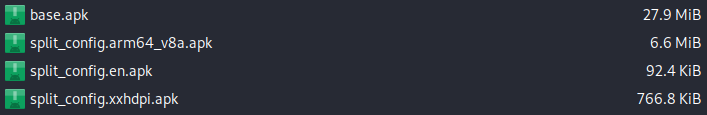
\includegraphics[width=0.7\linewidth]{../../images/connect-iq-apks}
    \caption{Connect IQ - Pulled apk files}
    \label{fig:connect-iq-apks}
\end{figure}
I installed the app on the phone and used $ADB$ to pull the apk files, that are presented in Figure~\ref{fig:connect-iq-apks}.
The app consists of multiple files, but the main one is \texttt{base.apk}.
It contains all JVM bytecode, which is the main focus of the analysis.
I decompiled the app with JADX decompiler\footnote{\url{https://github.com/skylot/jadx}}.

The app is obfuscated.
It is a good practice as it makes the app size smaller and makes it more difficult to reverse engineer.
I was interested to find the code responsible for downloading the app to the phone and sending it to the watch.
Searching with several keywords, I was not able to find any code that would be responsible for checking the certificate of the downloaded app.
I was looking for names such as the library that was used to sign the app, SHA1, RSA\@.

Assuming that the app is checking the certificate, it is not necessary for the phone to check it as well.
This is way it should be even safer, as the phone would be an additional attack surface.
With this conclusion, I decided to experiment later with the installation of an app that was not signed by the store in section~\ref{app-sideloading}.
\section{Static analysis}

\section{Sniffing the traffic}
To analyze the network security, I tried to sniff the traffic between the phone and Garmin servers.
I decided to use mitmproxy\footnote{\url{https://mitmproxy.org/}}.
When dynamically analyzing the app, there are two opitons.
Either use an emulator or a real device.
Emulator usually offers more flexibility and is easier to manipulate.
However, it does not have access to Bluetooth, which is necessary to test the app.
For this reason, I used a real device.
- linux hotspot + mitmproxy - problem with certificates.
Two options to solve the problem:
- Rooted phone
- Modify the app

The minimum supported Android version is 7.
Those versions require root access to add certificates supported by applications.
Another option is to modify the app to accept user added certificates.

\subsection*{Attempt 1 - Android Unpinner}
Use Android Unpinner - \footnote{\url{https://github.com/mitmproxy/android-unpinner}}

The app starts when connected to mitmproxy.
However, when trying to log in, it goes back to the welcome screen.
**Not possible to log in**.

\subsection*{Attempt 2 — manually modify the apk and sign again}

Using Apktool\footnote{\url{https://apktool.org/}} to unpack the app, modify, and pack again, align zip file and sign with a debug key.

After installing the app, there are some errors with missing resources.
I did not investigate it further.

\subsection*{Attempt 3 — only resign the app.}
Just resigning the app with a debug key.
The app starts, but when trying to log in it seems to work the same as the app from the attempt \#1.

\subsection*{Attempt 4 — use rooted phone}
I used my old, no longer used phone — Samsung S20.
To root the phone, I followed the instructions found on the XDA Forums\footnote{\url{https://xdaforums.com/t/how-to-exynos-snapdragon-root-s20-series-and-upgrade-firmware.4079353/}}.

\section{Network security,}
Based on the traffic that went through mitmproxy:

Used domains:
- `sso.garmin.com` - Qualys SSl Labs analysis: **grade B**
- server supports **TLS 1.1**
- `diauth.garmin.com` - Qualys SSl Labs analysis: **grade A**

\begin{figure}[h]
    \centering
    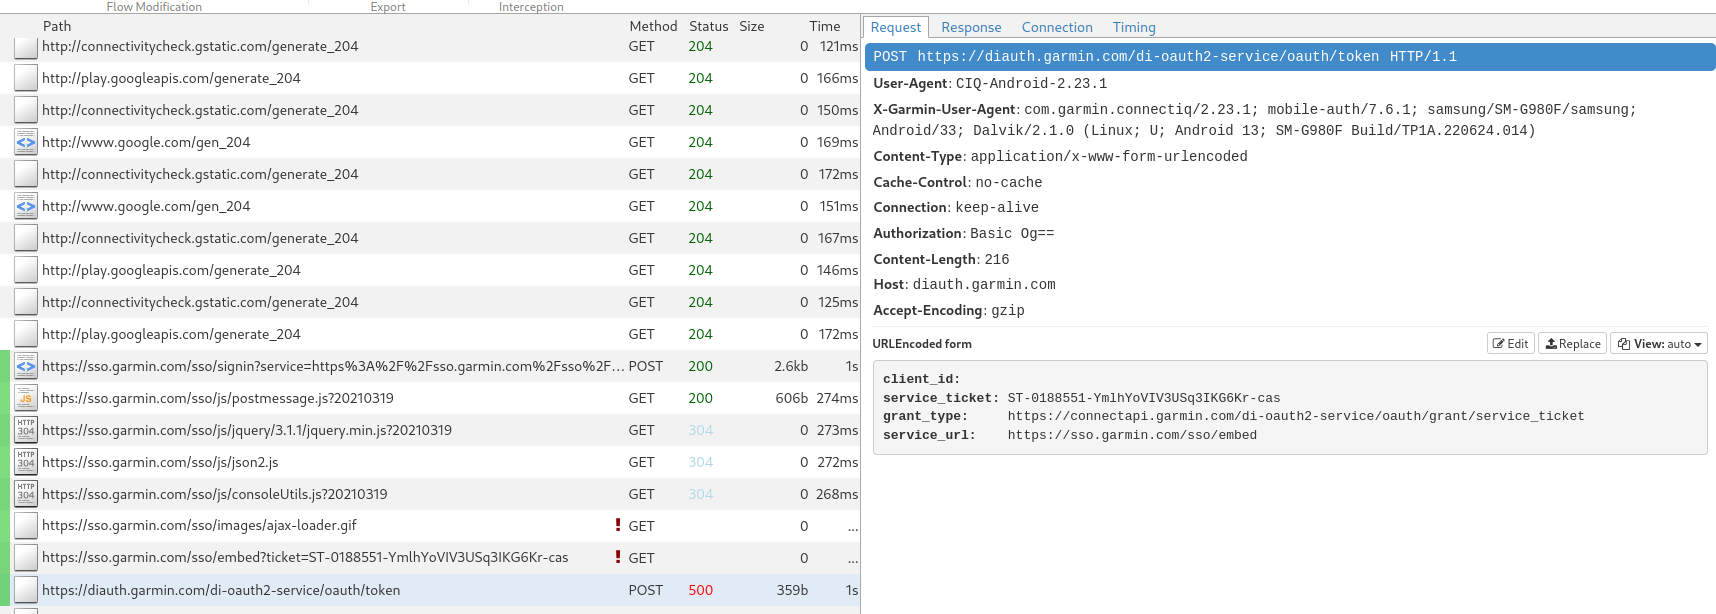
\includegraphics[width=1\linewidth]{../../images/mitmproxy unpinner}
    \caption{Sniffed traffic}
    \label{fig:mitmproxy-unpinner}
\end{figure}

The store displays content that can be added by the users.
The developer creates a description of the app, screenshots, and other information.
Other users can comment on the app.
I looked into it, to see how it is handled.
If the text was parsed by the app, it could be a potential vector of attack.
However, it seems that everything is sent as a plain text, without any parsing on the phone.

\section{Communication between the watch and the phone}
I considered analyzing the communication between the watch and the phone.
However, it uses Bluetooth LE Secure Connections.

\section{App sideloading}
\label{app-sideloading}
- can we install an app that is not signed up by the store?
- app signed up only by the developer can be install through the cable, but not through the store
- the watch is probably checking the certificate
- it suggests that the Bluetooth API for app installation requires the app to be signed by the store - good thing
